\documentclass[tikz]{standalone}
\usepackage{pgfplots}
\pgfplotsset{compat=1.15}
\usepackage{mathrsfs}
\usetikzlibrary{arrows,calc}
\usepackage{tkz-euclide}

\pagestyle{empty}

\definecolor{AngleClr}{rgb}{0,0.39215686274509803,0}
\definecolor{ShapeClr}{rgb}{0.6,0.2,0}

\begin{document}

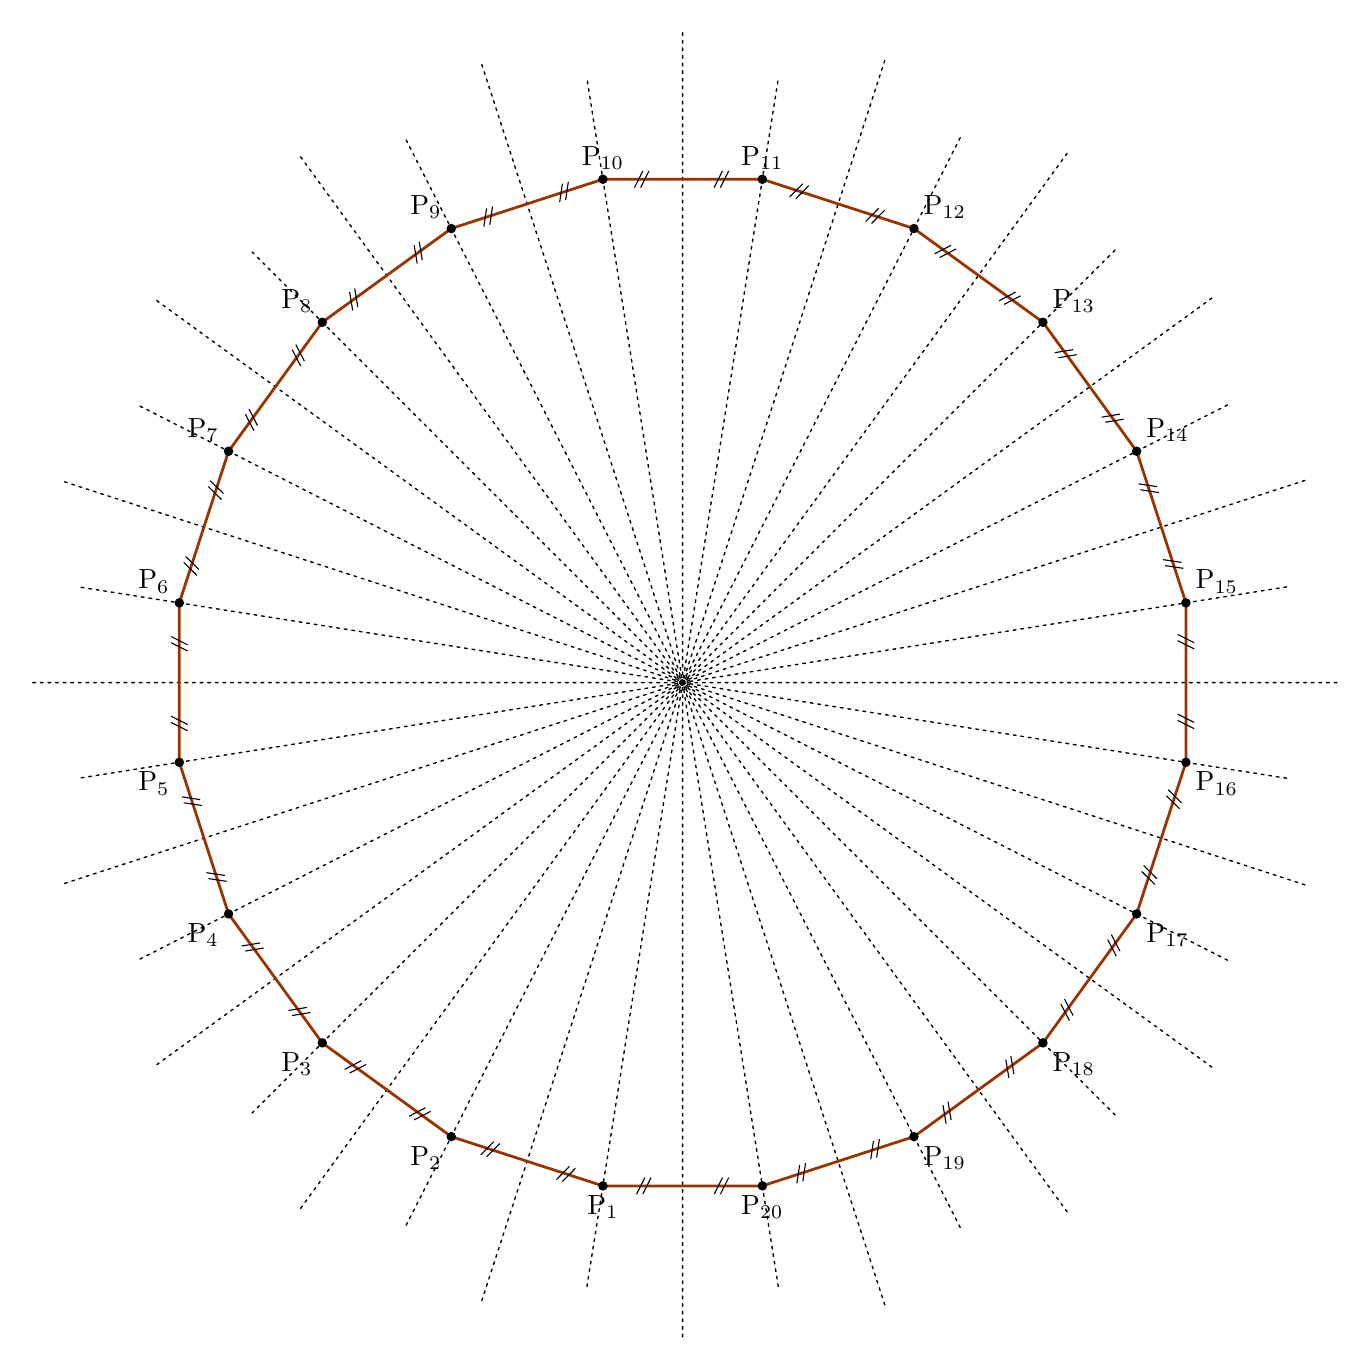
\begin{tikzpicture}[scale=.75]
\tkzSetUpLine[line width=1pt,color=black]
\tkzSetUpPoint[fill=black]

\tkzDefPoints{0/0/P0,2.7/0/P1}

\tkzDefRegPolygon[side,sides=20](P0,P1)

\tkzDefMidPoint(P1,P2) \tkzGetPoint{M1}
\tkzDefMidPoint(P2,P3) \tkzGetPoint{M2}
\tkzDefMidPoint(P3,P4) \tkzGetPoint{M3}
\tkzDefMidPoint(P4,P5) \tkzGetPoint{M4}
\tkzDefMidPoint(P5,P6) \tkzGetPoint{M5}
\tkzDefMidPoint(P6,P7) \tkzGetPoint{M6}
\tkzDefMidPoint(P7,P8) \tkzGetPoint{M7}
\tkzDefMidPoint(P8,P9) \tkzGetPoint{M8}
\tkzDefMidPoint(P9,P10) \tkzGetPoint{M9}
\tkzDefMidPoint(P10,P11) \tkzGetPoint{M10}
\tkzDefMidPoint(P11,P12) \tkzGetPoint{M11}
\tkzDefMidPoint(P12,P13) \tkzGetPoint{M12}
\tkzDefMidPoint(P13,P14) \tkzGetPoint{M13}
\tkzDefMidPoint(P14,P15) \tkzGetPoint{M14}
\tkzDefMidPoint(P15,P16) \tkzGetPoint{M15}
\tkzDefMidPoint(P16,P17) \tkzGetPoint{M16}
\tkzDefMidPoint(P17,P18) \tkzGetPoint{M17}
\tkzDefMidPoint(P18,P19) \tkzGetPoint{M18}
\tkzDefMidPoint(P19,P20) \tkzGetPoint{M19}
\tkzDefMidPoint(P20,P1) \tkzGetPoint{M20}


\tkzFillPolygon[fill=white](P1,P2,P3,P4,P5,P6,P7,P8,P9,P10,P11,P12,P13,P14,P15,P16,P17,P18,P19,P20)

\tkzDrawSegments[line width=0.5pt,color=black,dashed,dash pattern=on 1pt off 1.75pt,add=0.1 and 0.1](P1,P11 P2,P12 P3,P13 P4,P14 P5,P15 P6,P16 P7,P17 P8,P18 P9,P19 P10,P20)

\tkzDrawSegments[line width=0.5pt,color=black,dashed,dash pattern=on 1pt off 1.75pt,add=0.15 and 0.15](M1,M11 M2,M12 M3,M13 M4,M14 M5,M15 M6,M16 M7,M17 M8,M18 M9,M19 M10,M20)

\tkzDrawPolygon[color=ShapeClr](P1,P2,P3,P4,P5,P6,P7,P8,P9,P10,P11,P12,P13,P14,P15,P16,P17,P18,P19,P20)
\tkzDrawPoints[size=3](P1,P2,P3,P4,P5,P6,P7,P8,P9,P10,P11,P12,P13,P14,P15,P16,P17,P18,P19,P20)
\tkzLabelPoint[below](P1){$\rm P_1$}
\tkzLabelPoint[below](P2){$\rm P_{20}$}
\tkzLabelPoint[below right](P3){$\rm P_{19}$}
\tkzLabelPoint[below right](P4){$\rm P_{18}$}
\tkzLabelPoint[below right](P5){$\rm P_{17}$}
\tkzLabelPoint[below right](P6){$\rm P_{16}$}
\tkzLabelPoint[above right](P7){$\rm P_{15}$}
\tkzLabelPoint[above right](P8){$\rm \rm P_{14}$}
\tkzLabelPoint[above right](P9){$\rm \rm P_{13}$}
\tkzLabelPoint[above right](P10){$\rm P_{12}$}
\tkzLabelPoint[above](P11){$\rm P_{11}$}
\tkzLabelPoint[above](P12){$\rm P_{10}$}
\tkzLabelPoint[above left](P13){$\rm P_9$}
\tkzLabelPoint[above left](P14){$\rm P_8$}
\tkzLabelPoint[above left](P15){$\rm P_7$}
\tkzLabelPoint[above left](P16){$\rm P_6$}
\tkzLabelPoint[below left](P17){$\rm P_5$}
\tkzLabelPoint[below left](P18){$\rm P_4$}
\tkzLabelPoint[below left](P19){$\rm P_3$}
\tkzLabelPoint[below left](P20){$\rm P_2$}

\tkzMarkSegments[mark=s||,size=3](P1,M1 P2,M1 P2,M2 P3,M2 P3,M3 P4,M3 P4,M4 M4,P5 P5,M5 M5,P6 P6,M6 M6,P7 P7,M7 M7,P8 P8,M8 M8,P9 P9,M9 M9,P10 P10,M10 M10,P11 P11,M11 M11,P12 P12,M12 M12,P13 P13,M13 M13,P14 P14,M14 M14,P15 P15,M15 M15,P16 P16,M16 M16,P17 P17,M17 M17,P18 P18,M18 M18,P19 P19,M19 M19,P20 P20,M20 M20,P1)

\end{tikzpicture}

\end{document}
